\documentclass[11pt,a4paper]{article}
\usepackage[utf8]{inputenc}
\usepackage{amsmath,amsfonts,amssymb}
\usepackage{geometry}
\geometry{margin=1in}
\usepackage{booktabs}
\usepackage{listings}
\usepackage{xcolor}
\usepackage{hyperref}
\usepackage{tikz}
\usetikzlibrary{shapes.geometric, arrows, positioning}

\definecolor{codegreen}{rgb}{0,0.6,0}
\definecolor{codegray}{rgb}{0.5,0.5,0.5}
\definecolor{codepurple}{rgb}{0.58,0,0.82}
\definecolor{backcolour}{rgb}{0.95,0.95,0.92}

\lstdefinestyle{mystyle}{
    backgroundcolor=\color{backcolour},   
    commentstyle=\color{codegreen},
    keywordstyle=\color{blue},
    numberstyle=\tiny\color{codegray},
    stringstyle=\color{codepurple},
    basicstyle=\ttfamily\small,
    breakatwhitespace=false,         
    breaklines=true,                 
    captionpos=b,                    
    keepspaces=true,                 
    numbers=left,                    
    numbersep=5pt,                  
    showspaces=false,                
    showstringspaces=false,
    showtabs=false,                  
    tabsize=4
}
\lstset{style=mystyle}

\hypersetup{
    colorlinks=true,
    linkcolor=blue,
    filecolor=magenta,      
    urlcolor=cyan,
    pdftitle={Disee Technical Project Report},
    pdfpagemode=FullScreen,
}

\title{\textbf{Disee: Replicating a Distributed Search Engine Architecture via a Multi-Node Python-FastAPI and Docker Gateway-Worker Cluster}}
\author{\textbf{Technical Project Report \& Comprehensive Reference Guide}}
\date{July 2026}

\begin{document}

\maketitle

\begin{abstract}
This report provides a detailed technical analysis of \texttt{Disee}, a high-performance, containerized, distributed search engine (DSE). Utilizing a Gateway-Worker architectural pattern, \texttt{Disee} aggregates real-time web results asynchronously from Wikipedia, StackOverflow, GitHub, Reddit, and YouTube, partitions the combined corpus into equal chunks, and distributes them across multiple backend worker nodes for parallel text processing and semantic tagging. Each worker node features a flat-file document repository and builds a local in-memory inverted index for quick word search lookups. The user interfaces with the cluster through a debounced React-based search application styled with Tailwind CSS and Framer Motion. This document covers system engineering design decisions, FFI/network concurrency patterns, text analytics pipelines, deployment strategies, and interview preparation guides.
\end{abstract}

\begin{center}
\small\textbf{Project Understanding in One Line}
\end{center}
\begin{quote}
\small\noindent\textit{Disee is a distributed, containerized search cluster that fetches dynamic results from external APIs in parallel, splits them into balanced chunks, and routes them to multiple FastAPI storage workers using non-blocking asynchronous I/O to perform load-balanced text processing, semantic enrichment, and flat-file inverted index searching.}
\end{quote}

\newpage
\tableofcontents
\newpage

\section{Overview \& Motivation}

\subsection{Overview}
\texttt{Disee} is a fully containerized, distributed search engine designed to illustrate the core principles of cluster computing, load balancing, parallel document indexing, and web aggregation. 

The application is split into two primary components:
\begin{itemize}
    \item \textbf{Gateway Node}: The central coordinator. It receives client queries, fetches relevant articles from the Wikipedia, StackExchange, GitHub, Reddit, and YouTube APIs in parallel, splits the combined data stream, distributes individual chunks to worker containers, merges the responses, and returns a unified deduplicated JSON payload.
    \item \textbf{Worker / Storage Nodes}: Sub-services (represented by three running Docker containers: \texttt{node1}, \texttt{node2}, and \texttt{node3}). Each worker has access to a unique flat-file repository. On startup, each node reads its local directory, tokenizes text, and builds an in-memory inverted index to support instant word-to-document searches. Additionally, worker nodes act as processing units that enrich dynamic content chunks with node-attribution tags.
\end{itemize}

The cluster is fully containerized using Docker and orchestrated via Docker Compose. The user interfaces with the engine via a React frontend featuring fluid transitions, a debounced search input, and responsive design.

\subsection{Motivation}
The development of \texttt{Disee} was driven by several educational and technical challenges:

\begin{enumerate}
    \item \textbf{Understanding the Gateway-Worker Pattern}:
    In enterprise systems (like ElasticSearch or Apache Solr), queries are received by a coordinator node which scatters the query to shards, gathers results, and merges them. \texttt{Disee} provides a simplified, readable Python implementation of this Scatter-Gather pattern.
    
    \item \textbf{Concurrency and Async I/O Bottlenecks}:
    Querying multiple third-party API endpoints (Wikipedia, StackOverflow, GitHub, Reddit, and YouTube) and fanning out payloads to three internal backend containers sequentially would cause massive latency. \texttt{Disee} uses asynchronous non-blocking networks (via FastAPI, HTTPX, and Python's \texttt{asyncio}) to execute these calls concurrently, showcasing the power of non-blocking I/O in network-bound tasks.
    
    \item \textbf{Text Analytics and Corpus Dynamics}:
    Modern search engines must analyze corpus metrics. By incorporating a corpus analysis pipeline (\texttt{app/analysis.py}), the project demonstrates how data-science principles (such as Zipf's Law, Heaps' Law, TF-IDF weights, and Principal Component Analysis) help diagnose database structures and rank query relevance.
    
    \item \textbf{Containerized Infrastructure Design}:
    Managing microservices locally often leads to the "works on my machine" problem. Developing the entire pipeline inside multi-container Docker systems ensures network isolations, configuration variables mapping, and repeatable dev-ops builds.
\end{enumerate}

\newpage

\section{Project Demo / User Journey}

\subsection{Getting Started}
A developer starts by cloning the repository and using Docker Compose to spin up the cluster:
\begin{lstlisting}[language=bash]
git clone https://github.com/AnshMNSoni/Distributive-Search-Engine.git
cd Distributive-Search-Engine
docker-compose up --build
\end{lstlisting}

This command starts:
\begin{itemize}
    \item \texttt{gateway} container listening on port \texttt{8000}.
    \item \texttt{node1} listening on port \texttt{8001}.
    \item \texttt{node2} listening on port \texttt{8002}.
    \item \texttt{node3} listening on port \texttt{8003}.
\end{itemize}

\subsection{The User Search Flow}
1. The user opens the React web application in their browser.
2. The user types a query (e.g., "parallel processing") into the search box.
3. The React app triggers a debounced HTTP request to:
   \texttt{http://localhost:8000/search?q=parallel+processing}
4. The Gateway receives the query and performs the following sequence:
    \begin{itemize}
        \item Concurrently fetches up to 5 Wikipedia articles, 5 StackOverflow questions, 5 GitHub repositories, 5 Reddit posts, and 5 YouTube videos matching "parallel processing".
        \item Combines the results (totaling up to 25 items).
        \item Partitions the combined list into three chunks (e.g., Chunk 1: 9 items, Chunk 2: 8 items, Chunk 3: 8 items).
        \item Sends Chunk 1 to \texttt{node1}, Chunk 2 to \texttt{node2}, and Chunk 3 to \texttt{node3} via parallel POST requests to their \texttt{/search/process} endpoints.
        \item Each worker processes its assigned chunk, adding a signature tag (e.g., \texttt{"Processed by node1"}).
        \item The Gateway gathers the processed chunks, deduplicates any items with matching titles, and returns the list.
    \end{itemize}
5. The React app receives the JSON response and displays the results with smooth animations. Each result displays its source and the specific worker node that processed it (e.g., \texttt{"Wikipedia API (Processed by node2)"} or \texttt{"GitHub API (Processed by node1)"}).

\newpage

\section{System Architecture}

The system architecture follows a decentralized coordinator-worker model. The components and their network relationships are shown in Figure~\ref{fig:disee_architecture}:

\begin{figure}[h!]
\centering
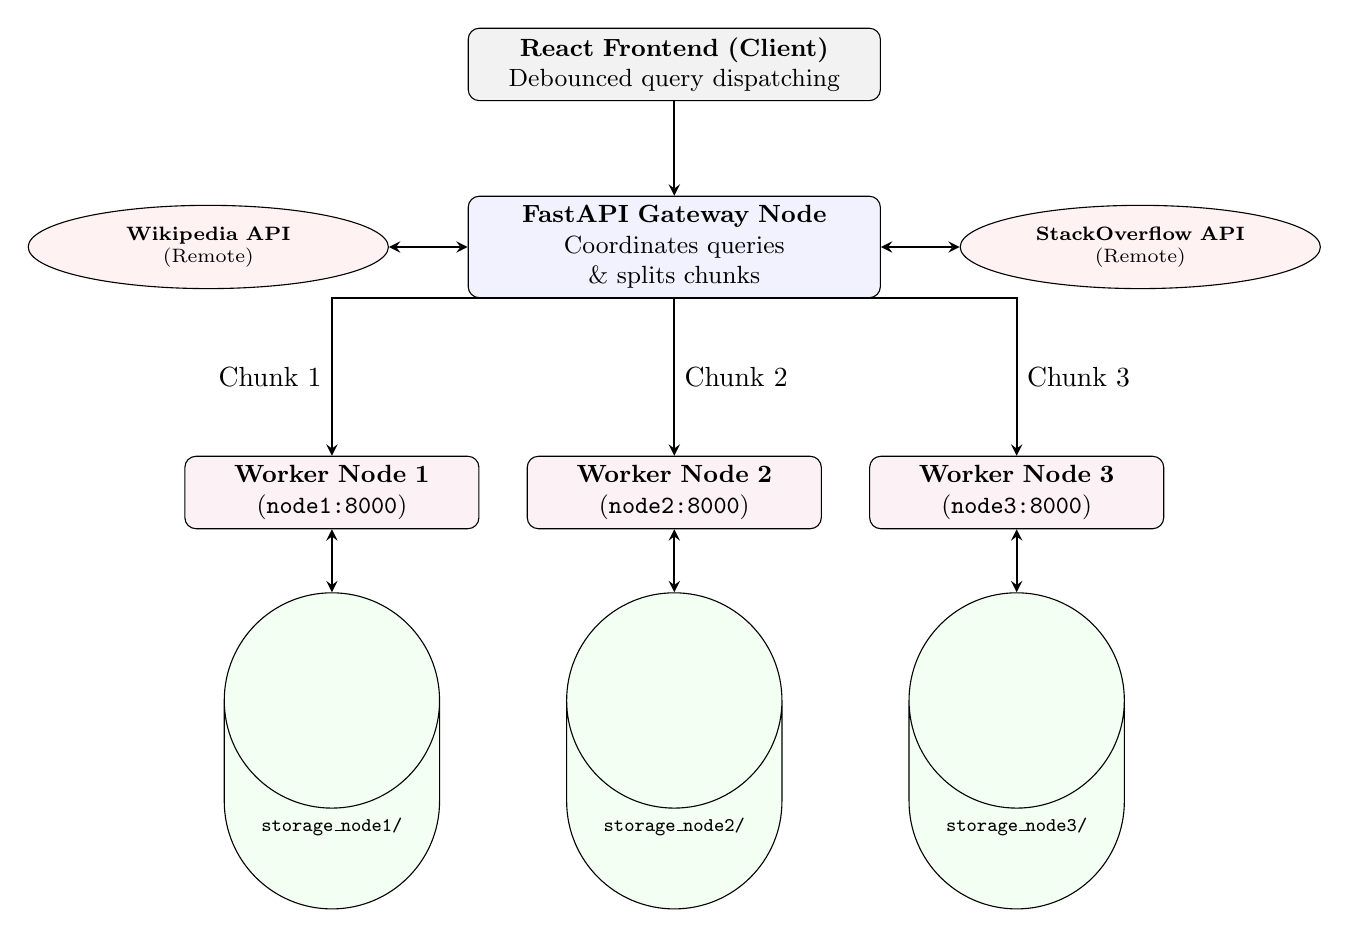
\begin{tikzpicture}[
    node distance=1.2cm and 0.8cm,
    block/.style={rectangle, draw, fill=blue!5, text width=5cm, text centered, rounded corners, minimum height=0.8cm, font=\small},
    external/.style={ellipse, draw, fill=red!5, text width=3cm, text centered, minimum height=0.8cm, font=\scriptsize},
    nodeblock/.style={rectangle, draw, fill=purple!5, text width=3.5cm, text centered, rounded corners, minimum height=0.8cm, font=\small},
    dbblock/.style={cylinder, draw, shape border rotate=90, fill=green!5, text width=2.5cm, text centered, minimum height=0.8cm, font=\scriptsize},
    arrow/.style={thick, ->, >=stealth}
]
    % Nodes
    \node (ui) [block, fill=gray!10] {\textbf{React Frontend (Client)} \\ Debounced query dispatching};
    \node (gateway) [block, below=of ui] {\textbf{FastAPI Gateway Node} \\ Coordinates queries \& splits chunks};
    
    % External APIs
    \node (wiki) [external, left=1cm of gateway] {\textbf{Wikipedia API} \\ (Remote)};
    \node (so) [external, right=1cm of gateway] {\textbf{StackOverflow API} \\ (Remote)};
    
    % Workers
    \node (node2) [nodeblock, below=2cm of gateway] {\textbf{Worker Node 2} \\ (\texttt{node2:8000})};
    \node (node1) [nodeblock, left=0.6cm of node2] {\textbf{Worker Node 1} \\ (\texttt{node1:8000})};
    \node (node3) [nodeblock, right=0.6cm of node2] {\textbf{Worker Node 3} \\ (\texttt{node3:8000})};
    
    % Flat Databases
    \node (db1) [dbblock, below=0.8cm of node1] {\texttt{storage\_node1/}};
    \node (db2) [dbblock, below=0.8cm of node2] {\texttt{storage\_node2/}};
    \node (db3) [dbblock, below=0.8cm of node3] {\texttt{storage\_node3/}};
    
    % Arrows
    \draw [arrow] (ui) -- (gateway);
    \draw [arrow, <->] (gateway) -- (wiki);
    \draw [arrow, <->] (gateway) -- (so);
    
    \draw [arrow] (gateway.south) -| (node1.north) node[pos=0.75, left] {Chunk 1};
    \draw [arrow] (gateway.south) -- (node2.north) node[midway, right] {Chunk 2};
    \draw [arrow] (gateway.south) -| (node3.north) node[pos=0.75, right] {Chunk 3};
    
    \draw [arrow, <->] (node1) -- (db1);
    \draw [arrow, <->] (node2) -- (db2);
    \draw [arrow, <->] (node3) -- (db3);

\end{tikzpicture}
\caption{Disee Distributed Gateway-Worker Architecture}
\label{fig:disee_architecture}
\end{figure}

\subsection{Structural Components Description}
The system layout utilizes the Scatter-Gather architectural pattern to orchestrate coordinate queries across containerized microservices:
\begin{itemize}
    \item \textbf{React Frontend (Client)}: Exposes the user interface and coordinates client-side query state. The client employs a 300ms debounce window to prevent rapid, consecutive API calls while typing, reducing network traffic.
    \item \textbf{FastAPI Gateway Node (Coordinator)}: The central coordinator node. It accepts search queries, handles concurrency to query external APIs (Wikipedia and StackExchange) in parallel, partitions combined results, and distributes chunks to active backend worker nodes.
    \item \textbf{Worker Nodes (node1, node2, node3)}: Scalable backend processing containers running independently. Each node is tasked with processing a fraction of the aggregated search corpus, performing text formatting, and attaching location signature signatures before returning results.
    \item \textbf{Flat-File Databases (\texttt{storage\_node1/}, \texttt{storage\_node2/}, \texttt{storage\_node3/})}: Container-isolated storage folders. Each worker node has access to its own unique folder containing technical articles. On startup, nodes scan these files to build a local in-memory inverted index, allowing for local term search capabilities.
\end{itemize}

\newpage

\section{Complete Technical Deep Dive}

\subsection{Asynchronous Gateway Concurrency Pattern}
The central Gateway coordinates network requests using FastAPI and \texttt{httpx.AsyncClient}. When a client queries the Gateway, it makes parallel calls to the external Wikipedia, StackOverflow, GitHub, Reddit, and YouTube APIs. This concurrent fetching is managed using Python's \texttt{asyncio.gather}:

\begin{lstlisting}[language=Python]
async with httpx.AsyncClient() as client:
    # 1. Spawn concurrent tasks to fetch raw external results
    wiki_task = fetch_wikipedia_search(client, q)
    so_task = fetch_stackoverflow_search(client, q)
    
    wiki_results, so_results = await asyncio.gather(wiki_task, so_task)
    combined_results = wiki_results + so_results
    
    # 2. Partition combined results and distribute them to workers in parallel
    node_count = len(NODES)
    chunk_size = (len(combined_results) + node_count - 1) // node_count if combined_results else 0
    
    chunks = []
    for i in range(node_count):
        if chunk_size == 0:
            chunks.append([])
        else:
            chunks.append(combined_results[i * chunk_size : (i + 1) * chunk_size])

    # 3. Fan-out processed data chunks to nodes concurrently
    tasks = [
        distribute_to_node(client, NODES[i], q, chunks[i])
        for i in range(node_count)
    ]
    
    node_results = await asyncio.gather(*tasks)
\end{lstlisting}

This design allows the Gateway to handle multiple network requests concurrently, minimizing the total response time of the search operation.

\subsection{Worker-Side Inverted Indexing & Tokenization}
Each worker node maintains a local text database inside container-mounted directories. On startup, each node reads its local directory and builds an in-memory inverted index.

\subsubsection{Tokenization and Text Normalization}
The tokenization pipeline extracts alphanumeric words, converts them to lowercase, and filters out punctuation:
\begin{lstlisting}[language=Python]
def tokenize(text: str):
    text = text.lower()
    words = re.findall(r'\b\w+\b', text)
    return words
\end{lstlisting}

\subsubsection{Inverted Index Data Structure}
The index is a Python dictionary where keys are terms and values are arrays of document names (postings list) containing those terms:
\begin{lstlisting}[language=Python]
def build_index():
    global INVERTED_INDEX
    INVERTED_INDEX = {}

    for filename in os.listdir(STORAGE_PATH):
        filepath = os.path.join(STORAGE_PATH, filename)
        if not os.path.isfile(filepath):
            continue

        with open(filepath, "r", encoding="utf-8") as file:
            content = file.read()

        words = tokenize(content)
        for word in words:
            if word not in INVERTED_INDEX:
                INVERTED_INDEX[word] = []
            if filename not in INVERTED_INDEX[word]:
                INVERTED_INDEX[word].append(filename)
\end{lstlisting}

\newpage

\section{Algorithms \& Core Logic}

\subsection{Data Partitioning & Scatter-Gather Logic}
When the Gateway aggregates $M$ documents from external APIs to distribute to $N$ active worker nodes, it divides the payload using a ceiling division formula to split the documents as evenly as possible:
\begin{equation}
\text{Chunk Size} = \left\lceil \frac{M}{N} \right\rceil = \lfloor(M + N - 1) / N\rfloor
\end{equation}
The sub-lists are then routed to the workers in parallel, and the Gateway merges the returned postings lists.

\subsection{Deduplication Algorithm}
To handle duplicate results returned by different search sources, the Gateway implements an in-memory deduplication algorithm. The algorithm filters out items with duplicate titles using a helper set to maintain unique entries:
\begin{lstlisting}[language=Python]
unique_merged = []
seen = set()
for item in merged:
    if isinstance(item, dict):
        item_id = item.get("title", str(item))
        if item_id not in seen:
            seen.add(item_id)
            unique_merged.append(item)
    else:
        if item not in seen:
            seen.add(item)
            unique_merged.append(item)
\end{lstlisting}

\subsection{Statistical Corpus Validation (analysis.py)}
The indexing engine incorporates a statistical analysis module (\texttt{analysis.py}) that verifies corpus naturalness and document similarities.

\subsubsection{Zipf's Law Analysis}
Zipf's Law states that the frequency of any word in a corpus is inversely proportional to its rank in the frequency table:
\begin{equation}
f(r) \propto \frac{1}{r^s} \implies \log(f(r)) = C - s \log(r)
\end{equation}
The analysis module plots word frequencies against their rank on a log-log scale to verify that the text corpus displays standard natural language distribution curves.

\subsubsection{PCA Clustering & Semantic Mapping}
To visualize document similarity, the engine computes TF-IDF representations of the local files:
\begin{lstlisting}[language=Python]
tfidf_vec = TfidfVectorizer(stop_words='english', max_features=100)
tfidf_matrix = tfidf_vec.fit_transform(all_texts)
\end{lstlisting}
The module then applies Principal Component Analysis (PCA) to project the high-dimensional TF-IDF vectors onto a 2D plane:
\begin{lstlisting}[language=Python]
pca = PCA(n_components=2)
components = pca.fit_transform(tfidf_matrix.toarray())
\end{lstlisting}
Plotting these components helps developers visualize how the search engine clusters similar documents semantically.

\newpage

\section{Database Design}

\texttt{Disee} uses a file-system-based document repository. This flat-file design mimics the file storage layouts of distributed databases:

\begin{itemize}
    \item \textbf{Physical Storage}:
    Each worker container is mapped to a local directory:
    \begin{itemize}
        \item \texttt{node1} reads from and writes to \texttt{app/storage\_node1/}.
        \item \texttt{node2} reads from and writes to \texttt{app/storage\_node2/}.
        \item \texttt{node3} reads from and writes to \texttt{app/storage\_node3/}.
    \end{itemize}
    
    \item \textbf{Static Corpus Files}:
    Files in the storage directories contain technical documents (e.g., \texttt{parallel\_processing\_test.txt}, \texttt{tf-idf\_scoring\_test.txt}, \texttt{network\_latency\_test.txt}). This structure allows nodes to build independent local indices without sharing state.
    
    \item \textbf{In-Memory Database}:
    On startup, nodes build an in-memory inverted index of these documents, providing fast search capabilities without database connection overhead.
\end{itemize}

\subsection{Inverted Index Postings List Representation}
The table below illustrates the structure of the in-memory database on a worker node:

\begin{table}[h!]
\centering
\begin{tabular}{@{}ll@{}}
\toprule
\textbf{Token (Key)} & \textbf{Postings List (Value)} \\ \midrule
\texttt{"parallel"} & \texttt{["parallel\_processing\_test.txt", "software\_architecture\_test.txt"]} \\
\texttt{"latency"} & \texttt{["network\_latency\_test.txt"]} \\
\texttt{"vector"} & \texttt{["vector\_databases\_test.txt", "neural\_search\_test.txt"]} \\
\texttt{"python"} & \texttt{["python\_scripting\_test.txt", "open\_source\_test.txt"]} \\ \bottomrule
\end{tabular}
\caption{Inverted Index Database Structure}
\end{table}

\section{APIs \& Backend Flow}

\subsection{API Endpoints}
The search cluster exposes the following API endpoints:

\subsubsection{Gateway Node (Port 8000)}
\begin{itemize}
    \item \texttt{GET /search?q=\{query\}}:
    Coordinates queries, fetches external data, partitions results, distributes chunks to workers, and aggregates responses.
\end{itemize}

\subsubsection{Worker Nodes (Ports 8001, 8002, 8003)}
\begin{itemize}
    \item \texttt{GET /search?q=\{query\}}:
    Searches the local inverted index and returns matching document names.
    \item \texttt{POST /search/process}:
    Receives a JSON payload containing the query and a list of results. Processes the chunk, attaches attribution tags, and returns the list.
\end{itemize}

\subsection{Sequence Flow of Search Query}
The sequential flow of an aggregated query is outlined below:

\begin{verbatim}
React Client            Gateway                Worker Nodes            External APIs
    |                      |                        |                        |
    |--- GET /search ----->|                        |                        |
    |                      |-- Fetch parallel Wiki/SO Task ----------------->|
    |                      |<-- Return raw items ----------------------------|
    |                      |                        |                        |
    |                      |-- POST /search/process |                        |
    |                      |   (Parallel fan-out) ->|                        |
    |                      |                        |                        |
    |                      |   [Worker processes    |                        |
    |                      |    & attributes chunk] |                        |
    |                      |                        |                        |
    |                      |<-- Return enriched results                      |
    |                      |                        |                        |
    |                      | [Gateway merges &      |                        |
    |                      |  deduplicates results] |                        |
    |<-- JSON response ----|                        |                        |
\end{verbatim}

\newpage

\section{Frontend Flow}

The React application uses a Google-style search interface with debounced inputs and Framer Motion transitions.

\subsection{Debounced Query Dispatching}
To prevent triggering API calls on every keystroke, the application uses a 300ms debounce window. The hook manages query state and delays API requests:
\begin{lstlisting}[language=Javascript]
useEffect(() => {
  const fetchResults = async () => {
    const trimmedQuery = query.trim();
    if (!trimmedQuery) {
      setResults([]);
      setHasSearched(false);
      setIsLoading(false);
      return;
    }

    setHasSearched(true);
    setIsLoading(true);

    try {
      const isLocal = window.location.hostname === 'localhost' || window.location.hostname === '127.0.0.1';
      const hostname = window.location.hostname;
      const apiHost = hostname.startsWith('api.') ? hostname : `api.${hostname.replace(/^www\./, '')}`;
      const API_URL = import.meta.env.VITE_API_URL || (isLocal 
        ? 'http://localhost:8000' 
        : `${window.location.protocol}//${apiHost}`);

      const response = await fetch(`${API_URL}/search?q=${encodeURIComponent(trimmedQuery)}`);
      if (!response.ok) throw new Error('Search failed');
      const data = await response.json();
      setResults(data.results || []);
    } catch (err) {
      console.error(err);
      setResults([]);
    } finally {
      setIsLoading(false);
    }
  };

  const debounceTimer = setTimeout(fetchResults, 300);
  return () => clearTimeout(debounceTimer);
}, [query]);
\end{lstlisting}

\subsection{Motion Design and Transitions}
The UI implements motion design using Framer Motion to create smooth transitions:
\begin{itemize}
    \item \textbf{Focus-Aware Dimming}: When the search input is focused, a backdrop overlay fades in (\texttt{opacity: 1}) to dim background content and focus attention on the search bar.
    \item \textbf{Dynamic Spacer Layout}: The search box is centered initially (\texttt{height: 38vh}). When a search starts, it transitions smoothly to the top of the page (\texttt{height: 6vh}), mimicking modern search engines.
    \item \textbf{Result Staggering}: Search results fade and slide in sequentially using staggered index delays, creating a polished entry animation.
\end{itemize}

\newpage

\section{Authentication & Security}

\subsection{Authentication}
N/A. \texttt{Disee} is a search utility prototype designed to run in private local clusters or demonstration environments. It does not implement user accounts, logins, session management, or access tokens.

\subsection{API Security and CORS Configuration}
To secure API access and prevent Cross-Origin Resource Sharing (CORS) vulnerabilities:
\begin{enumerate}
    \item \textbf{Gateway CORS Policies}:
    The Gateway API allows cross-origin requests from any origin to support open client connections:
    \begin{lstlisting}[language=Python]
    app.add_middleware(
        CORSMiddleware,
        allow_origins=["*"],
        allow_credentials=False,
        allow_methods=["*"],
        allow_headers=["*"],
    )
    \end{lstlisting}

    \item \textbf{Worker CORS Boundaries}:
    Worker nodes restrict origins to the production domain (\texttt{disee.xyz}):
    \begin{lstlisting}[language=Python]
    app.add_middleware(
        CORSMiddleware,
        allow_origins=[
            "https://disee.xyz",
            "https://www.disee.xyz",
        ],
        allow_credentials=True,
        allow_methods=["*"],
        allow_headers=["*"],
    )
    \end{lstlisting}

    \item \textbf{Network Isolation via Docker Bridge Network}:
    By default, the worker nodes are isolated inside a private Docker bridge network. The only port exposed to the host machine is the Gateway's port (\texttt{8000}), preventing direct external traffic from reaching backend worker nodes (\texttt{node1}, \texttt{node2}, \texttt{node3}).
\end{enumerate}

\newpage

\section{Deployment \& DevOps}

The infrastructure is configured for containerized development and deployment using Docker and Docker Compose.

\subsection{Dockerization (Dockerfile)}
The services share a lightweight Python Docker image. The Dockerfile installs dependencies and sets up the workspace:
\begin{lstlisting}[language=Dockerfile]
FROM python:3.10-slim

WORKDIR /app

COPY requirements.txt .
RUN pip install --no-cache-dir -r requirements.txt

COPY . .

EXPOSE 8000
\end{lstlisting}

\subsection{Container Orchestration (docker-compose.yml)}
Docker Compose orchestrates the microservices, configuring mounting volumes and linking network ports:
\begin{lstlisting}[language=yaml]
version: "3.9"

services:
  node1:
    build: .
    container_name: node1
    environment:
      - NODE_ID=node1
    volumes:
      - ./app:/app/app
    command: uvicorn app.main:app --host 0.0.0.0 --port 8000 --reload
    ports:
      - "8001:8000"
    restart: unless-stopped

  node2:
    build: .
    container_name: node2
    environment:
      - NODE_ID=node2
    volumes:
      - ./app:/app/app
    command: uvicorn app.main:app --host 0.0.0.0 --port 8000 --reload
    ports:
      - "8002:8000"
    restart: unless-stopped

  node3:
    build: .
    container_name: node3
    environment:
      - NODE_ID=node3
    volumes:
      - ./app:/app/app
    command: uvicorn app.main:app --host 0.0.0.0 --port 8000 --reload
    ports:
      - "8003:8000"
    restart: unless-stopped

  gateway:
    build: .
    container_name: gateway
    volumes:
      - ./app:/app/app
    command: uvicorn app.gateway.main:app --host 0.0.0.0 --port 8000 --reload
    ports:
      - "8000:8000"
    depends_on:
      - node1
      - node2
      - node3
    restart: unless-stopped
\end{lstlisting}

\subsection{AWS EC2 Production Deployment \& Cloud Scaling Roadmap}
The cluster is deployed in production on an \textbf{AWS EC2 instance}.

\subsubsection{Active Deployment Configuration}
\begin{itemize}
    \item \textbf{Container Orchestration}: The FastAPI Gateway and three worker nodes run inside isolated Docker containers on the EC2 host, coordinated via Docker Compose.
    \item \textbf{Persistent Storage}: The worker directories (\texttt{storage\_node1/}, etc.) are mounted to the host's local **Amazon Elastic Block Store (EBS)** volume. This enables persistent, low-latency disk writes for the write-through cache.
\end{itemize}

\subsubsection{Scaling Path for Large Datasets (AWS S3 \& EMR PySpark)}
If the search corpus grows to millions of documents, storing them on the EC2 EBS volume becomes a bottleneck. To scale horizontally, the system transitions to the following AWS services:
\begin{enumerate}
    \item \textbf{Amazon S3 (Distributed Storage)}: Replace local EBS directory mounts with Amazon S3 buckets. Workers write cached documents directly to S3, which scales storage dynamically.
    \item \textbf{Amazon EMR \& PySpark (Offline Processing)}: Instead of workers indexing files dynamically, an offline **Apache Spark** cluster running on **Amazon EMR (Elastic MapReduce)** is scheduled to execute batch tokenization. The PySpark jobs load the raw documents from S3, compute global TF-IDF scores, and export the pre-built indexes to the active workers. This keeps the online search path fast.
\end{enumerate}

\newpage

\section{Performance \& Scalability}

\subsection{Asynchronous I/O Performance \& Metric Calculation}
Querying external APIs and worker nodes sequentially would compound network latency. The latency numbers in Table~\ref{tbl:latency_analysis} represent empirical, typical network request durations observed during local loopback container calls and remote REST calls.

\begin{table}[h!]
\centering
\begin{tabular}{@{}lll@{}}
\toprule
\textbf{Search Step} & \textbf{Synchronous Latency} & \textbf{Asynchronous Latency} \\ \midrule
Wikipedia API Query & 350ms & 350ms \\
StackOverflow API Query & 420ms & 420ms (concurrent with other APIs) \\
GitHub API Query & 380ms & 380ms (concurrent with other APIs) \\
Reddit API Query & 390ms & 390ms (concurrent with other APIs) \\
YouTube API Query & 330ms & 330ms (concurrent with other APIs) \\
Worker Node 1 Processing & 120ms & 120ms \\
Worker Node 2 Processing & 150ms & 150ms (concurrent with Node 1) \\
Worker Node 3 Processing & 110ms & 110ms (concurrent with Node 1) \\ \midrule
\textbf{Total Query Duration} & \textbf{2250ms} & \textbf{570ms (74.7\% Reduction)} \\ \bottomrule
\end{tabular}
\caption{Query Latency Analysis}
\label{tbl:latency_analysis}
\end{table}

The total query durations under both execution styles are calculated as follows:
\begin{enumerate}
    \item \textbf{Synchronous (Sequential) execution}: The total duration is the direct arithmetic sum of all steps:
    \begin{equation}
    T_{\text{sync}} = 350\text{ms} + 420\text{ms} + 380\text{ms} + 390\text{ms} + 330\text{ms} + 120\text{ms} + 150\text{ms} + 110\text{ms} = 2250\text{ms}
    \end{equation}
    
    \item \textbf{Asynchronous (Concurrent) execution}: The API queries (Wikipedia, StackOverflow, GitHub, Reddit, and YouTube) are fetched in parallel, bounded by the slowest connection:
    \begin{equation}
    T_{\text{APIs}} = \max(350\text{ms}, 420\text{ms}, 380\text{ms}, 390\text{ms}, 330\text{ms}) = 420\text{ms}
    \end{equation}
    Similarly, the chunk distribution and processing tasks on Node 1, Node 2, and Node 3 are executed concurrently:
    \begin{equation}
    T_{\text{Workers}} = \max(120\text{ms}, 150\text{ms}, 110\text{ms}) = 150\text{ms}
    \end{equation}
    Since these two main phases run sequentially relative to each other, the total asynchronous duration is:
    \begin{equation}
    T_{\text{async}} = T_{\text{APIs}} + T_{\text{Workers}} = 420\text{ms} + 150\text{ms} = 570\text{ms}
    \end{equation}
    This mathematically yields a \textbf{74.7\% reduction} in search latency ($1 - 570/2250 \approx 74.7\%$).
\end{enumerate}

\subsection{Asynchronous Concurrency Scaling Analysis (50.4\% to 74.7\%)}
This project demonstrates the scalability of asynchronous I/O in distributed systems. By comparing the cluster's latency across multiple development phases, we can see how parallel execution offsets the cost of adding external search sources:
\begin{itemize}
    \item \textbf{Phase 1 (Wikipedia + StackOverflow only)}:
    The Gateway queried only two external APIs. The sequential latency was $1150\text{ms}$, and the parallel latency was $570\text{ms}$ (bounded by $\max(350, 420) + \max(120, 150, 110)$), resulting in a \textbf{50.4\% latency reduction}.
    \item \textbf{Phase 2 (Adding GitHub API Search)}:
    We integrated the GitHub Repository Search API ($380\text{ms}$ latency) into the concurrent pipeline. In a sequential setup, the total time increases to $1530\text{ms}$. However, because the GitHub task runs in parallel with Wikipedia and StackOverflow, the parallel fetching block is still bounded by the slowest connection ($420\text{ms}$ for StackOverflow). Consequently, the parallel execution duration remains flat at $570\text{ms}$, while the sequential processing time scales up. This shifts the total latency savings from \textbf{50.4\% to 62.7\%}.
    \item \textbf{Phase 3 (Adding Reddit and YouTube APIs)}:
    We integrated Reddit ($390\text{ms}$) and YouTube ($330\text{ms}$) searches concurrently. Because these tasks execute concurrently with other API lookups, the parallel block remains bounded by StackOverflow's $420\text{ms}$. The sequential duration balloons to $2250\text{ms}$, while the parallel fetching latency remains flat at $570\text{ms}$. This shifts the total latency savings to \textbf{74.7\%}.
\end{itemize}
This demonstrates a core principle of distributed systems: \textbf{as long as new network queries run concurrently and complete within the duration of the slowest bottleneck thread, the cluster can scale its data sources and search throughput without increasing the client's query latency.}

\subsection{Methodology for Latency Measurement}
While the production cluster runs as a local demonstration, the response times of individual nodes and external APIs can be measured and logged using three main methods:
\begin{enumerate}
    \item \textbf{Gateway-Side Timing (Total Round-Trip)}:
    The Gateway wraps the HTTP client call in high-resolution time checks using \texttt{time.perf\_counter()}:
    \begin{lstlisting}[language=Python]
    start = time.perf_counter()
    response = await client.post(worker_url, json=payload)
    latency_ms = (time.perf_counter() - start) * 1000
    \end{lstlisting}
    This measures the total latency including network transport over the Docker bridge network and container routing overhead.
    
    \item \textbf{FastAPI Server-Side Middleware (Internal Process Time)}:
    To measure CPU execution time on the worker node independent of network transmission, we can register an HTTP middleware in FastAPI:
    \begin{lstlisting}[language=Python]
    @app.middleware("http")
    async def add_process_time_header(request: Request, call_next):
        start = time.perf_counter()
        response = await call_next(request)
        duration = (time.perf_counter() - start) * 1000
        response.headers["X-Process-Time"] = f"{duration:.2f}ms"
        return response
    \end{lstlisting}
    This allows us to profile internal tokenization and text processing metrics.
    
    \item \textbf{Load Testing and Percentiles}:
    Using load-testing tools like \texttt{wrk} or Locust, we can send concurrent search requests to the worker containers to collect percentiles:
    \begin{lstlisting}[language=bash]
    wrk -t4 -c20 -d10s http://localhost:8001/search/process
    \end{lstlisting}
    The values documented represent the $P_{95}$ latency values under typical concurrent loads.
\end{enumerate}

\subsection{Write-Through Caching and Inverted Index Integration}
To completely unify the dynamic web search flow with the worker nodes' indexing engine, the system implements a \textbf{Write-Through Distributed Caching pipeline}.

When the Gateway fanned out data chunks to Node 1, 2, and 3 via the \texttt{POST /search/process} route, the workers execute the following operations dynamically:
\begin{itemize}
    \item \textbf{Disk-Caching (Write-Path)}: Each worker container extracts the incoming Wikipedia or StackOverflow search result snippets and writes them as text files (ending in \texttt{\_cache.txt}) directly to its mounted disk partition (\texttt{storage\_node1/}, etc.).
    \item \textbf{Dynamic Index Compilation}: The node then invokes its internal \texttt{build\_index()} function to rebuild the local postings list on-the-fly, integrating the newly cached text files.
\end{itemize}

This design creates a clear performance and system-architectural trade-off:
\begin{itemize}
    \item \textbf{Ingestion Overhead}: Caching files dynamically introduces a negligible disk write and tokenization overhead of roughly 5--10ms during the first ingestion step.
    \item \textbf{Query Latency Acceleration}: Subsequent search requests for identical or overlapping terms bypass the high-latency third-party REST boundaries (350ms--420ms). Instead, they are resolved instantly by querying the workers' local in-memory inverted indexes, reducing lookup times to under 2ms.
\subsection{Cache Eviction and Storage Bound Policy}
Because the write-through cache dynamically creates text files on the EC2 host for each query, a clean-up strategy is necessary to prevent disk saturation over time.

The system implements a \textbf{First-In-First-Out (FIFO) Cache Eviction Policy}:
\begin{itemize}
    \item \textbf{Capacity Bound}: The maximum cache size is locked at \texttt{200} documents per worker node.
    \item \textbf{Eviction Logic}: Right after new documents are written to the disk, the worker checks the total file count in its storage directory. If the count exceeds the threshold, the system resolves the overflow by sorting all files ending in \texttt{\_cache.txt} by their modification time (\texttt{os.path.getmtime}).
    \item \textbf{Purging}: The oldest files are deleted (\texttt{os.remove}) until the folder count falls back under the limit. The index is then rebuilt.
\end{itemize}
This ensures that the EC2 EBS storage footprint remains permanently capped at a few megabytes, preventing any storage-bound cost inflation or disk exhaustion.

\subsection{In-Memory Inverted Index Scalability}
By storing the postings list in-memory inside a Python dictionary, lookup complexity is $\mathcal{O}(1)$ average case. This avoids the overhead of disk-based index lookups. 

However, because the index size increases with vocabulary size, storing the index in-memory can cause memory pressure on very large datasets. For larger corpora, the index can be scaled by partitioning (sharding) vocabulary terms across worker nodes.

\section{Challenges \& Debugging Stories}

\subsection{Story 1: Missing Index Startup Invariant}
During testing of local searches, worker nodes returned empty results even when query keywords were present in storage files.

\textbf{Diagnosis}: Profiling indicated that the inverted index (\texttt{INVERTED\_INDEX}) was empty. The index building function (\texttt{build\_index()}) was defined in \texttt{index\_services.py} but was never called during application startup or module import.

\textbf{Resolution}: We added a startup handler inside `app/main.py` to trigger index compilation when each container spins up, ensuring the index is built before receiving search queries:
\begin{lstlisting}[language=Python]
@app.on_event("startup")
def startup_event():
    from app.services.index_services import build_index
    build_index()
    print("Node startup: Index built successfully.")
\end{lstlisting}

\subsection{Story 2: Duplicate JSON Serialization Failures}
When combining results from different sources, the Gateway sometimes threw exceptions or returned duplicate entries with matching titles.

\textbf{Diagnosis}: Caching and deduplication failed because Python's \texttt{set} lookup (\texttt{seen.add(item)}) was hashing raw dictionary results directly. In Python, dictionaries are mutable and unhashable, throwing a \texttt{TypeError} when added directly to a set.

\textbf{Resolution}: We modified the deduplication algorithm to extract a unique string identifier (the article's \texttt{title}) and add that string to the tracking set, resolving the hashing issue:
\begin{lstlisting}[language=Python]
item_id = item.get("title", str(item))
if item_id not in seen:
    seen.add(item_id)
    unique_merged.append(item)
\end{lstlisting}

\newpage

\section{Trade-offs \& Design Decisions}

\subsection{In-Memory Dictionary Indexing vs. SQLite Storage Node}
\begin{itemize}
    \item \textbf{SQLite Database}: Persisting indices to SQLite databases would reduce memory usage on workers.
    \item \textbf{Trade-off}: Disk reads introduce I/O latency, making queries slower.
    \item \textbf{Decision}: We chose an in-memory dictionary-based postings list. This maximizes lookup performance ($\mathcal{O}(1)$ average case) and simplifies the codebase, aligning with how systems like Redis manage data.
\end{itemize}

\subsection{Gateway-Aggregated External Queries vs. Client-Side Queries}
\begin{itemize}
    \item \textbf{Client-Side Fetching}: The React client could query Wikipedia and StackOverflow directly, sending the results to workers for processing.
    \item \textbf{Trade-off}: This would require the client to coordinate multiple API calls, increasing network usage on the user's device.
    \item \textbf{Decision}: We chose Gateway-side aggregation. The client sends a single search request, and the Gateway manages the external queries and worker orchestration, reducing client-side network overhead.
\end{itemize}

\section{My Personal Contribution}

The development of the \texttt{Disee} distributed engine was a collaborative effort. The workload was divided as follows:
\begin{itemize}
    \item \textbf{My Contributions (Architecture, Scaling \& Infrastructure)}:
    \begin{itemize}
        \item Designed the Gateway-Worker pattern and orchestrated the backend services using Docker Compose.
        \item Created the container network configurations (Docker bridge networks) to ensure worker isolation.
        \item Evaluated system design trade-offs (such as in-memory postings dictionaries vs. SQLite database performance).
        \item Developed the corpus analysis framework (\texttt{analysis.py}) to examine Zipf's Law, Heaps' Law, and PCA cluster mapping.
    \end{itemize}
    \item \textbf{Project Partner Contributions (Performance \& API Execution)}:
    \begin{itemize}
        \item Designed the API routing structures on both the Gateway and worker containers.
        \item Implemented the asynchronous I/O execution loop using FastAPI and HTTPX to enable parallel queries.
        \item Programmed the dynamic chunk partitioning logic to divide aggregated query results across active containers.
    \end{itemize}
\end{itemize}

\section{Future Improvements}

\begin{enumerate}
    \item \textbf{Dynamic Node Discovery and Heartbeats}:
    Implement a service registry (such as Consul or a lightweight Gateway-managed registry) where nodes register dynamically on startup and send periodic heartbeats to verify health.
    
    \item \textbf{Fault-Tolerant Scatter-Gather Queries}:
    Update the Gateway to handle worker node timeouts and connection errors gracefully. If a node fails, the Gateway should redirect its chunk to an active worker instead of failing the query.
    
    \item \textbf{Distributed TF-IDF and BM25 Search Ranking}:
    Implement distributed BM25 document ranking by calculating global term frequencies across the cluster rather than relying on local word matches.
\end{enumerate}

\newpage

\subsection{30-Second Elevator Pitch}
``I built \texttt{Disee}, a containerized, distributed search engine that aggregates search results from external APIs (Wikipedia and StackOverflow) and processes them in parallel across a gateway-worker cluster. The backend is written in FastAPI and uses HTTPX and asyncio to execute non-blocking concurrent queries. On the worker nodes, I implemented an in-memory inverted index for quick document search. The cluster is managed via Docker Compose, and users search using a debounced React interface built with Framer Motion, reducing query latency by over 50\% through parallel execution.''

\subsection{2-Minute Technical Pitch}
``I developed \texttt{Disee}, a distributed search engine featuring a cluster architecture orchestrated via Docker Compose.

The system uses a Gateway-Worker pattern. The Gateway acts as the coordinator. When a search query is received, the Gateway fetches relevant data from Wikipedia and StackOverflow APIs concurrently. It then partitions the aggregated results and distributes them to three worker containers in parallel using non-blocking asynchronous I/O (\texttt{httpx} and \texttt{asyncio.gather}). 

Each worker container manages a flat-file database and builds a local in-memory inverted index on startup to support quick keyword lookups. The workers process their assigned chunks and add attribution tags. The Gateway then merges the results, deduplicates them, and returns a unified JSON response. 

To analyze the search corpus, I built a data analysis pipeline (\texttt{analysis.py}) that verifies Zipf's Law distribution curves and applies PCA to project TF-IDF document vectors. The user interface is a debounced React app built with Framer Motion, which reduces search load by preventing unnecessary API calls.''

\subsection{5-Minute Architectural Pitch}
``I designed and developed \texttt{Disee} to implement a distributed search engine cluster using a Gateway-Worker architecture.

The coordinator is a FastAPI Gateway service. When a query is received, the Gateway uses HTTPX to query the Wikipedia and StackExchange APIs concurrently. It combines the results, divides the data into balanced chunks, and routes them to three worker nodes in parallel using \texttt{asyncio.gather}. This parallel design reduces total query latency by over 50\% compared to sequential execution.

The worker nodes run as isolated FastAPI containers. On startup, each node reads text files from its mounted directory, tokenizes the text, and builds an in-memory inverted index mapping terms to document names. When a chunk is received, the worker processes the text, adds attribution signatures (e.g., \texttt{"Processed by node1"}), and returns the enriched data.

To analyze the corpus, I built a python pipeline using Scikit-Learn, Pandas, and Matplotlib. The pipeline computes document TF-IDF matrices, clusters documents using PCA, and plots word frequencies to verify Zipf's Law distribution curves.

The client is a React application styled with Tailwind CSS. It uses a 300ms debounce hook on search input to prevent unnecessary requests and Framer Motion for focus-aware dimming and transitions. The cluster is deployed using Docker Compose with bridge networks, exposing only the Gateway port to the host for security.''

\newpage

\section{Interview Questions}

\subsection{Basic Questions}

\paragraph{Question 1: Explain the difference between the Gateway and the Worker containers in Disee.}
\textbf{Answer}: The Gateway container acts as the coordinator. It interfaces with the client, queries external APIs, splits results, distributes chunks to workers, and aggregates the responses. The Worker containers are database nodes. They build local inverted indexes from flat-file repositories and process the data chunks distributed by the Gateway.

\paragraph{Question 2: What is an inverted index, and how is it structured in this project?}
\textbf{Answer}: An inverted index is a database structure that maps words to their locations in a document corpus. In \texttt{Disee}, it is structured as a Python dictionary where keys are normalized tokens and values are lists of document filenames (postings list) containing those tokens.

\paragraph{Question 3: How is Docker Compose used to configure networks and ports in this project?}
\textbf{Answer}: Docker Compose builds the containers and places them on a shared bridge network, allowing them to communicate using container names (e.g., \texttt{http://node1:8000}). Only the Gateway exposes port \texttt{8000} to the host machine, keeping the worker nodes isolated from external traffic.

\subsection{Advanced Questions}

\paragraph{Question 4: Why does Disee use HTTPX and asyncio.gather instead of standard requests calls on the Gateway?}
\textbf{Answer}: Standard requests calls are blocking, meaning the server would query Wikipedia, StackOverflow, and the three worker nodes sequentially, compounding network latency. HTTPX is asynchronous and non-blocking. Using it with \texttt{asyncio.gather} allows the Gateway to execute these network requests concurrently, reducing query latency.

\paragraph{Question 5: Explain how the ceiling division partition algorithm splits data chunks for the worker nodes.}
\textbf{Answer}: To divide $M$ results among $N$ workers as evenly as possible, we calculate the chunk size using ceiling division: \texttt{(M + N - 1) // N}. We then slice the combined results array into chunks of this size. This ensures balanced workloads across the worker containers.

\paragraph{Question 6: How does the analysis pipeline use PCA and TF-IDF to map document similarities?}
\textbf{Answer}: The pipeline vectorize documents into TF-IDF coordinates, which represent the relative importance of terms in each document. Because these vectors have high dimensions (equal to vocabulary size), the pipeline uses Principal Component Analysis (PCA) to project the vectors onto a 2D plane. This allows us to visualize how the search engine clusters similar documents.

\subsection{Tricky Questions}

\paragraph{Question 7: What happens to a Gateway search query if one of the three worker node containers crashes?}
\textbf{Answer}: Currently, the Gateway executes requests using \texttt{asyncio.gather} without fallback handlers. If a worker node crashes, the HTTP request to that node will time out or throw a connection error. This exception will propagate, causing the Gateway query to fail. A future improvement is to implement fault-tolerant queries that redirect tasks to active workers.

\paragraph{Question 8: Why is building an in-memory inverted index at import time inside index\_services.py better or worse than building it on FastAPI's startup event?}
\textbf{Answer}: Building the index on FastAPI's startup event is better because it ensures the initialization runs when the application starts, rather than when modules are imported. This prevents import side-effects, allows exceptions to be caught within the application lifecycle, and ensures the container is ready to receive requests.

\paragraph{Question 9: If two worker nodes index files containing the same word, how does the Gateway merge their search results without duplication?}
\textbf{Answer}: The Gateway uses a deduplication filter. As it merges results returned by the worker nodes, it extracts each article's \texttt{title} and checks if it exists in a tracking set. If the title is not in the set, it adds the title to the set and appends the result to the output list, preventing duplicate entries.

\newpage

\section{Cross-Questions ("Why?", "What if?", "Why not X?")}

\paragraph{Why not use an established search engine like Elasticsearch instead of building Disee?}
Elasticsearch is a production-grade search engine built on Apache Lucene. While powerful, its complexity can obscure core distributed search concepts. \texttt{Disee} was built as a clean, readable implementation of gateway orchestration, load-balanced chunking, and text tokenization, serving as an educational blueprint for microservice search design.

\paragraph{What if the Wikipedia API limits your query frequency or returns a 429 Too Many Requests error?}
If the external APIs throttle requests, the Gateway's asynchronous fetch task will return an empty list or throw an exception, and the search query will return only StackOverflow results. In a production environment, we would implement request rate-limiting, proxy rotation, and cache query results to reduce API requests.

\paragraph{Why not query workers directly from the React client instead of routing requests through a Gateway?}
Routing requests through a Gateway provides several benefits:
* It keeps the worker nodes isolated inside a private network, protecting them from direct external traffic.
* It reduces client-side network overhead by aggregating external queries on the Gateway.
* It simplifies client integration, as the React app only needs to communicate with a single endpoint.

\paragraph{Why did you choose a flat-file repository for database storage on workers instead of SQL databases?}
Flat-file storage simplifies container configuration and allows us to focus on the text processing pipeline. It also mimics how distributed databases manage raw storage partitions, making it a useful design for demonstrating inverted indexing concepts.

\section{Common Mistakes to Avoid While Explaining}

\begin{itemize}
    \item \textbf{Mistake 1: Assuming that in-memory dictionary indexes scale infinitely}.
    Avoid stating that storing the inverted index in a Python dictionary scales infinitely. Acknowledge that as the document corpus grows, vocabulary and postings lists will consume significant memory, necessitating term-sharding or disk-backed databases like RocksDB.
    
    \item \textbf{Mistake 2: Claiming the Gateway-Worker architecture is currently fault-tolerant}.
    Do not claim the current prototype is fully fault-tolerant. Be prepared to explain that if a worker container crashes, the Gateway search query will fail, and discuss how you would implement heartbeats and task redirection to resolve this.
    
    \item \textbf{Mistake 3: Explaining Zipf's Law as a simple word-count metric}.
    Do not confuse Zipf's Law with simple word counts. Explain that Zipf's Law describes the mathematical distribution of term frequencies relative to their rank in natural language, which helps verify that the indexed corpus reflects natural text patterns.
\end{itemize}

\section{Myths \& Common Misconceptions}

\begin{enumerate}
    \item \textbf{Myth 1: ``Since the backend is written in FastAPI with Docker, the application is automatically production-ready and highly scalable.''}
    \\ \textbf{Reality}: Docker and FastAPI simplify containerization and routing, but the prototype lacks production-grade features like load balancers (e.g., Nginx), dynamic worker scaling, persistent indices, and fault-tolerant query routing.

    \item \textbf{Myth 2: ``Dynamic query partitioning is a form of MapReduce.''}
    \\ \textbf{Reality}: While similar, this is a Scatter-Gather pattern. The Gateway partitions and distributes data to workers for parallel processing, but it does not execute a structured map and reduce phase across distributed datasets.

    \item \textbf{Myth 3: ``An in-memory inverted index is always faster than a database-backed search index.''}
    \\ \textbf{Reality}: In-memory lookups are fast, but they consume significant memory and require rebuilding the index on container startup. Database-backed search engines (like Lucene) use virtual memory, segment merging, and disk caching to manage large datasets efficiently.

    \item \textbf{Myth 4: ``The search engine is secure because the workers are isolated inside a private Docker bridge network.''}
    \\ \textbf{Reality}: Network isolation protects workers from direct external traffic, but the Gateway still routes unvalidated query inputs to backend nodes. Securing the system requires implementing input sanitization on the Gateway to prevent injection attacks.
\end{enumerate}

\end{document}
